\chapter{Exploration of atomistic predictions}
\label{chapter2}

Atomic interactions are the foundation on which many ML models---especially interatomic potential models---are built.
Accuracy is well-defined in quantum chemical methods via systematic convergence and comparison to experimental data, but wavefunction-based approaches are computationally expensive and are limited to system sizes of only a handful of atoms.
Measuring predictive accuracy is difficult when approximating the results of first principles computations for systems that exceed the size limitations of QM approaches.
This raises a vital question to the efficacy of ML models: how do we assess the reliability of atomistic neural network potential models for systems that exceed the size limitations of QM computations?

The scalability of NNP models stems from partitioning molecules into atomic components, characterized by their local chemical environment.
However, this introduces new challenges in generalization and transferability and, therefore, model reliability when exposed to new atomic interactions during inference.
This chapter serves as an assessment of the reliability of model predictions of molecular enery and atomistic energy contributions in ANAKIN-ME neural network potential models.
Section \ref{sec:ANI_predictions} contains a detailed look at the predictions of ANI neural networks from atomistic features to global properties and the measure of uncertainty used to determine the trustworthiness of a prediction.
The following section, \ref{sec:uncertainty_atomic_energies}, details the search for an improved metric of reliability in atomistic predictions.

\section{ANAKIN-ME Predictions}
\label{sec:ANI_predictions}

The ANI methodology provides a framework for atom-wise decomposition of molecular energies by using the atomic environment vector (AEV) representation to encode localized chemical interactions.
A decomposition approach allows for efficient, scalable predictions of energy for systems larger than the training data represents.
This is advantageous for simulating large systems, due to the size limitations of \textit{ab initio} computations.
The driving idea behind the AEV representation is that all atomic interactions within a system can be characterized by the localized environment. 
This neglects long-range interactions such as van der Waals forces and electrostatics, which are undoubtedly important for some systems, but has little influence on the predictive accuracy of single-point calculations of small organic molecules.
Corrective approaches to long-range interactions have been explored, such as ANI-MBIS-q \cite{ml_mm_santi_y_jonny2}, which considers long-range electrostatics using a separate, parallel network to predict partial charges.
For small, charge-neutral molecules, localized interactions encoded in the AEV have been shown to capture the relationship between molecular energy and atomic species and their positions \cite{ani-1, ani-1x, ani-2x}.

Though some partitioning schemes exist in quantum theory, such as Bader's Atoms in Molecules \cite{bader_aim}, there is no general consensus for decomposing the energy of a molecular system into a sum of atomic contributions.
The energy decomposition approach taken by ANI is a learned relationship decided by the individual atomic neural networks during training, explained in greater detail in Subsection \ref{subsec:total_E_sum_AEs}.
The uncertainty measure of predicted energies, referred to as the QBC, is defined in Subsection \ref{subsec:ANI_uncertainty}, followed by a case study in Subsection \ref{subsec:flaws_in_qbc} of the reliability of the QBC as a measure of empirical uncertainty in ANI predictions.

\subsection{Molecular Energy as a Sum of Atomic Contributions}
\label{subsec:total_E_sum_AEs}

The predicted molecular energy for a molecule input to an ANI model is computed as a sum of atomic contributions, given in Eqn. \ref{eq:total_E_sum_AEs}, where $E_{\text{Total}}$ is the molecular energy prediction and $\varepsilon_i$ is the atomic energy contribution for atom $i$.

\begin{equation}
    E_{\text{Total}} = \sum_{i}^{\text{atoms}} \varepsilon_i
    \label{eq:total_E_sum_AEs}
\end{equation}

To visualize atomic energy predictions, a small testing subset was created using the first conformer of each molecular formula in the ANI-1x training dataset.
This testing set, referred to as 1x-test ($N=$ 3,114), is used to explore some trends in predicted atomic energies for the carbon, hydrogen, nitrogen, and oxygen atom types across an ensemble of eight models.
Testing on this subset gives insight on the performance of ANI models for well-characterized systems, as this was the data used in training the model.
The ANI-1x and 2x potential models were trained using self-atomic energies (SAEs), where the predicted atomic energy values form a distribution centered at zero. 
This means that, by definition, each atom has either no net contribution to the molecular energy, or contributes an energy deviation that is relative to the baseline for that atom type.
The atomic energy contributions predicted by the ANI-2x model for C, H, N, and O atoms across the 1x-first test set are given in Figure \ref{fig:2x_ae_per_model}.

\begin{figure}[!h]
    \centering
    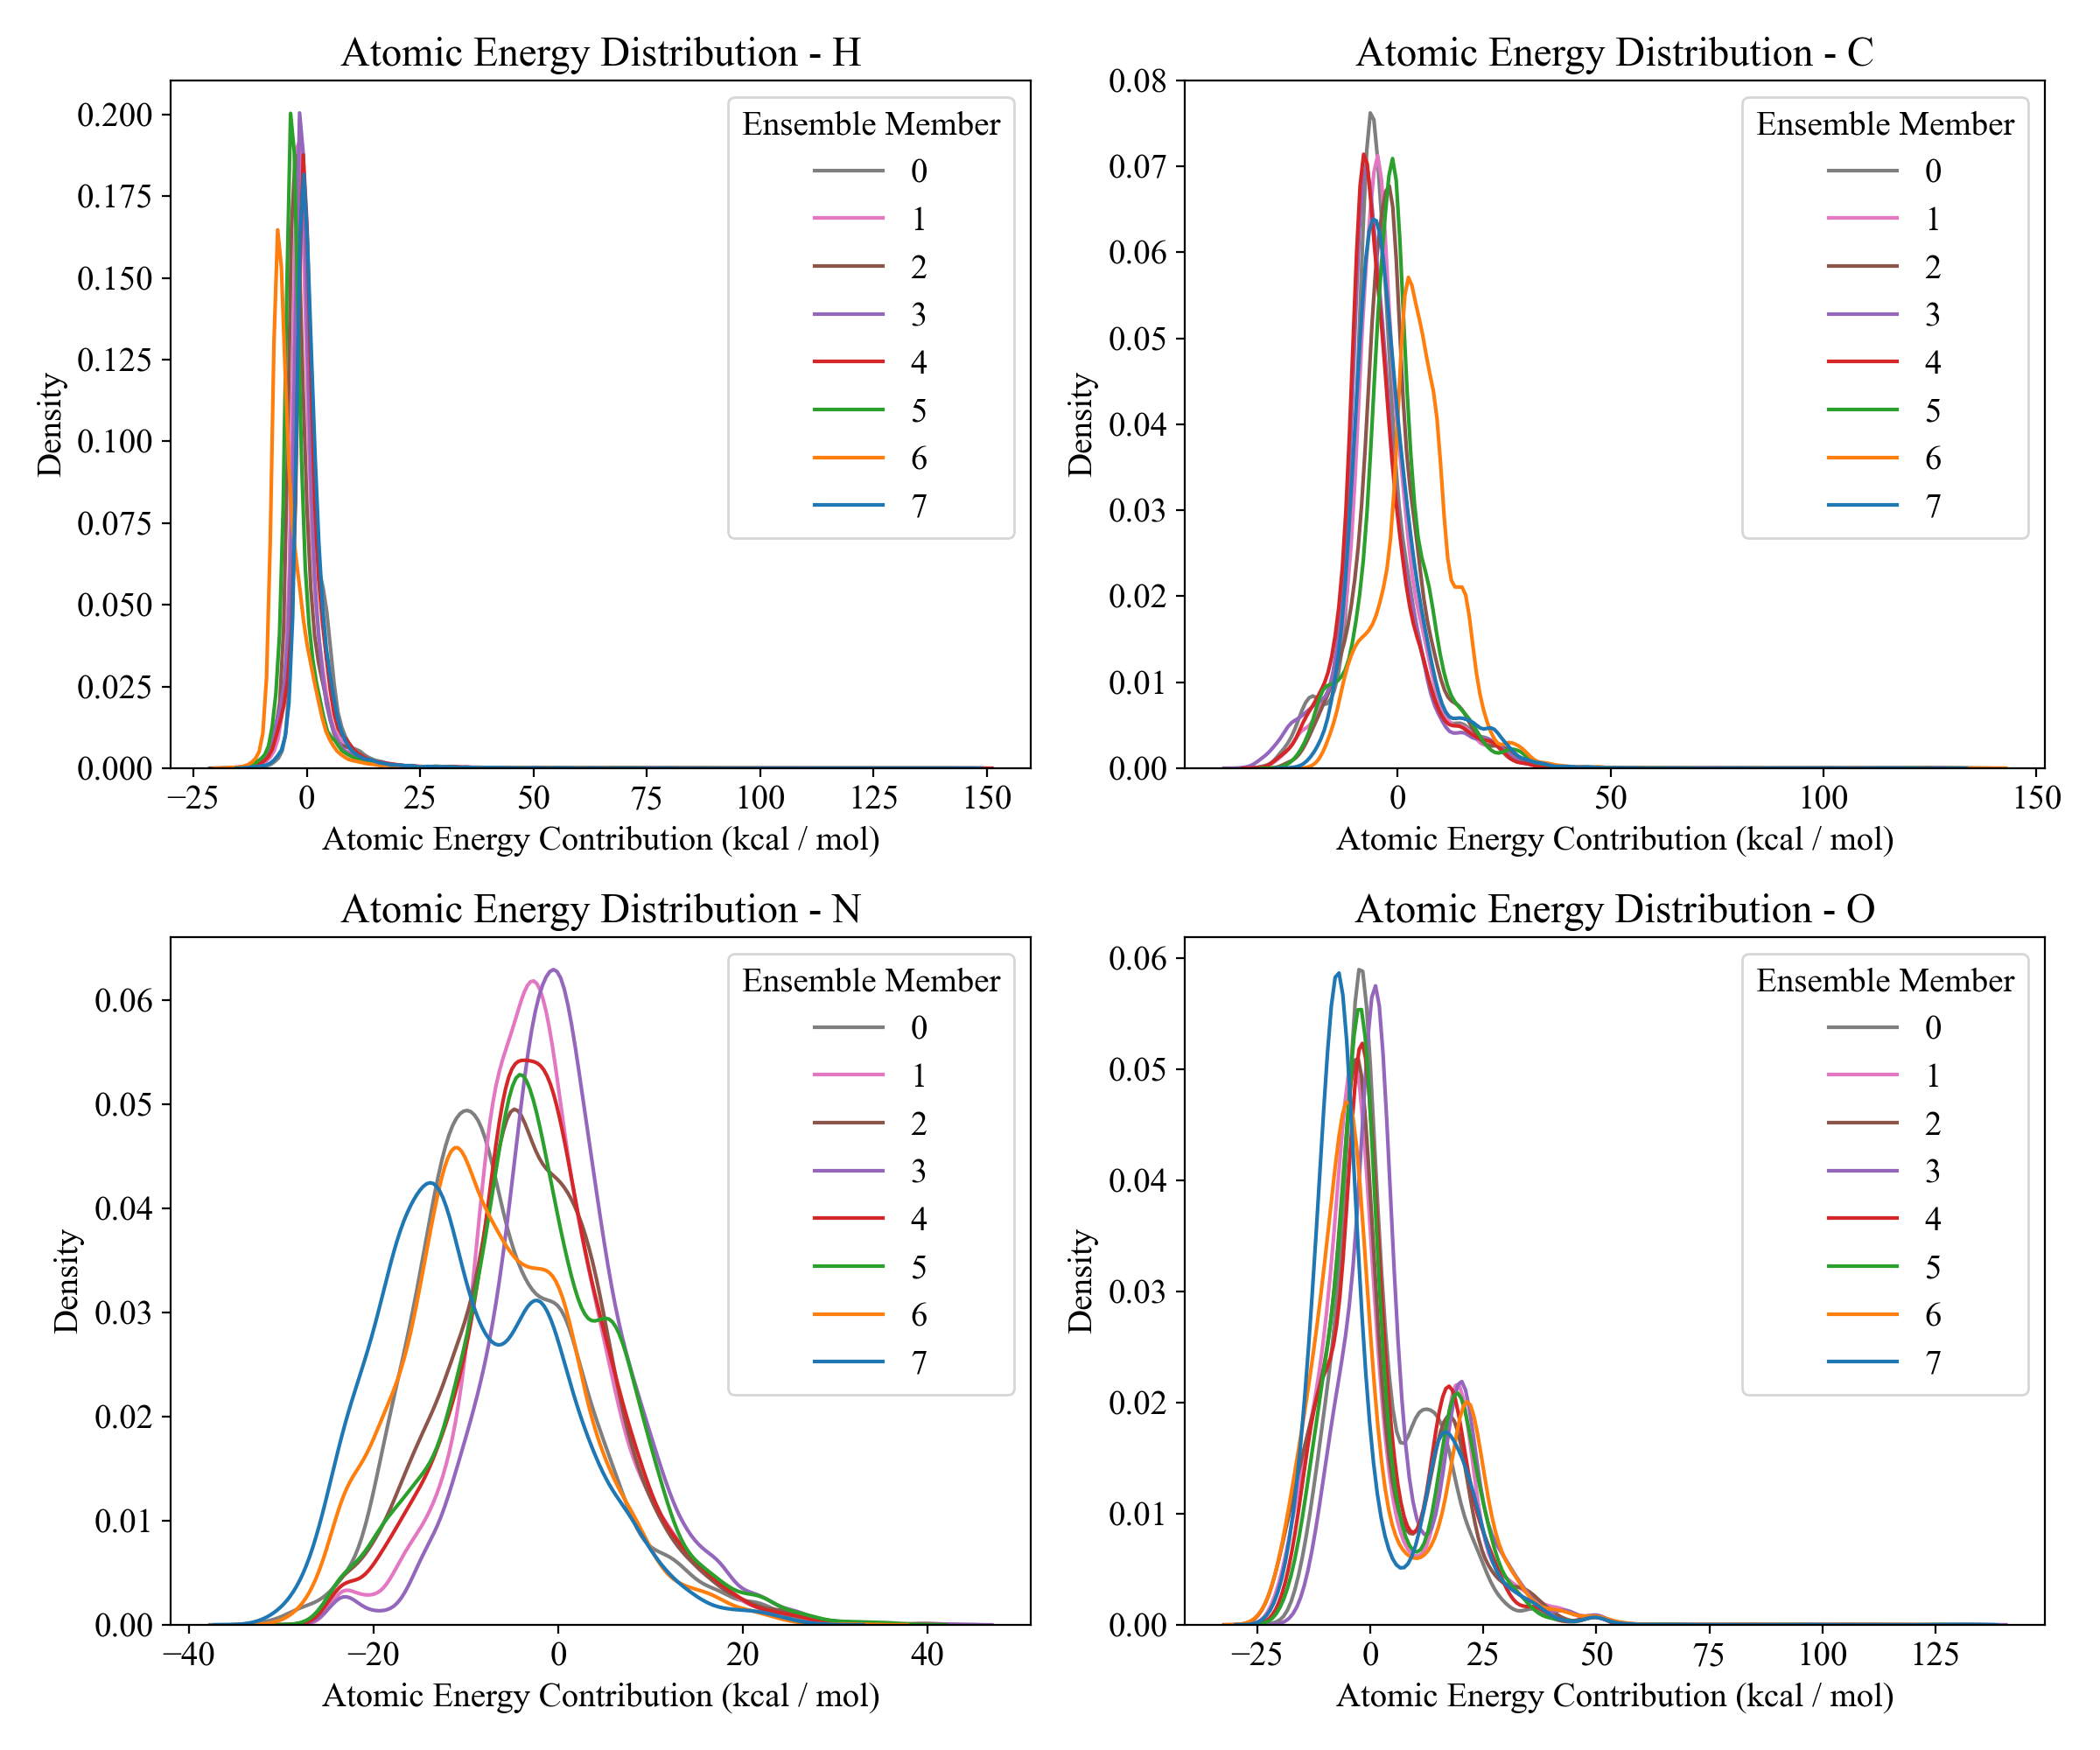
\includegraphics[width=1\linewidth]{Images/2x_outputs/2x_1x-first_ae-per-model.png}
    \caption[Atomic energies predicted by ANI-2x]{Per-model distribution of atomic energy contributions by atom type for the ANI-2x potential. Values shown in kcal/mol for HCNO atom types on the 1x-first subset.}
    \label{fig:2x_ae_per_model}
\end{figure}

Shifting atomic energies with SAEs causes the model to learn relative energy contributions rather than absolute values. 
Refined ANI models, such as ANI-2xr, are trained with slightly different hyperparameters.
The largest change between ANI-2x and 2xr is the removal of biases from neuron outputs; Eqn. \ref{eq:nn_eqn} shows the method for computing the weighted-sum output of each neuron ($y$) from the input ($x_i$) multiplied by its weight ($w_i$).
Traditionally, artificial neural networks use biases to output some value, even when the weighted sum of input values is close or equal to zero.
For interatomic potentials, if we pass a single atom with no neighbors through a network, we would expect to get exactly the energy of that atom in space with no other interacting particles.
By removing the biases from the species-specific networks, we can achieve this goal and add a bit more physicality to the behavior of the neural network outputs.
To replace the biases, we add a final shift to the output: the EnergyShifter.
This is a protocol within TorchANI which adds the ground state atomic energy (GSAE) to each atom, shifting the output values of the NNs toward physically meaningful values.
Ground state atomic energies are calculated at the level of theory used in producing training data from a neutrally charged atom isolated in space with the proper spin multiplicity (ensuring a ground-state electronic configuration).
Thus, the total energy prediction in ANI-2xr networks are computed as shown in Equation \ref{eq:total_E_GSAEs}.

\begin{equation}
    E_{\text{Total}} = \sum_{i}^{\text{atoms}} \varepsilon_i + \text{GSAE}_i
    \label{eq:total_E_GSAEs}
\end{equation}

Here, the total energy is a sum of atomic contributions as in Eqn. \ref{eq:total_E_sum_AEs}, and $\text{GSAE}_i$ is the ground state atomic energy for atom $i$, which shift the network outputs toward more physically meaningful values.
The ground state atomic energies for each atom in the ANI networks are given in \ref{appendix:GSAEs}.
In addition to the removal of biases and the replacement of self-atomic energies with GSAEs, ANI-2xr is trained with the addition of a simple, analytical xTB repulsion term \cite{xtb_repulsion}.
The inclusion of repulsion to the potential introduces more physical behavior in regions of the potential energy surface that are difficult to sample, namely when two atoms get very close together.
Equation \ref{eq:repulsion} shows the form of this repulsion term for two atoms, where $a$ and $b$ (with atomic numbers $A$ and $B$, respectively) separated by a distance $r_{ab}$. 
The parameters $Y_A$ and $Y_B$ define the magnitude of the repulsive term for their respective elements, $\alpha_{A}$ and $\alpha_{B}$ are element-specific parameters, and $k_{AB}$ is a small correction for very light elements (H, He) and equal to 3/2 in all other cases.

\begin{equation}
\label{eq:repulsion}
    E_{\text{rep}}(r_{ab}) = 
    \sum_{AB}\frac{{Y_{A} Y_{B}}}{r_{ab}}
    \exp \left( -\sqrt{\alpha_{A} \alpha_{B}} {(r_{ab})}^{k_{AB}} \right)
\end{equation}

The ANI-2xr atomic energy distribution for hydrogen, carbon, nitrogen, and oxygen are given in Fig. \ref{fig:2xr_ae_per_model} for an eight-membered ensemble.
Note here that the distributions have slightly different shapes, as well as being shifted far from the zero-centered ANI-2x distributions shown in Figure \ref{fig:2x_ae_per_model}.

\begin{figure}[H]
    \centering
    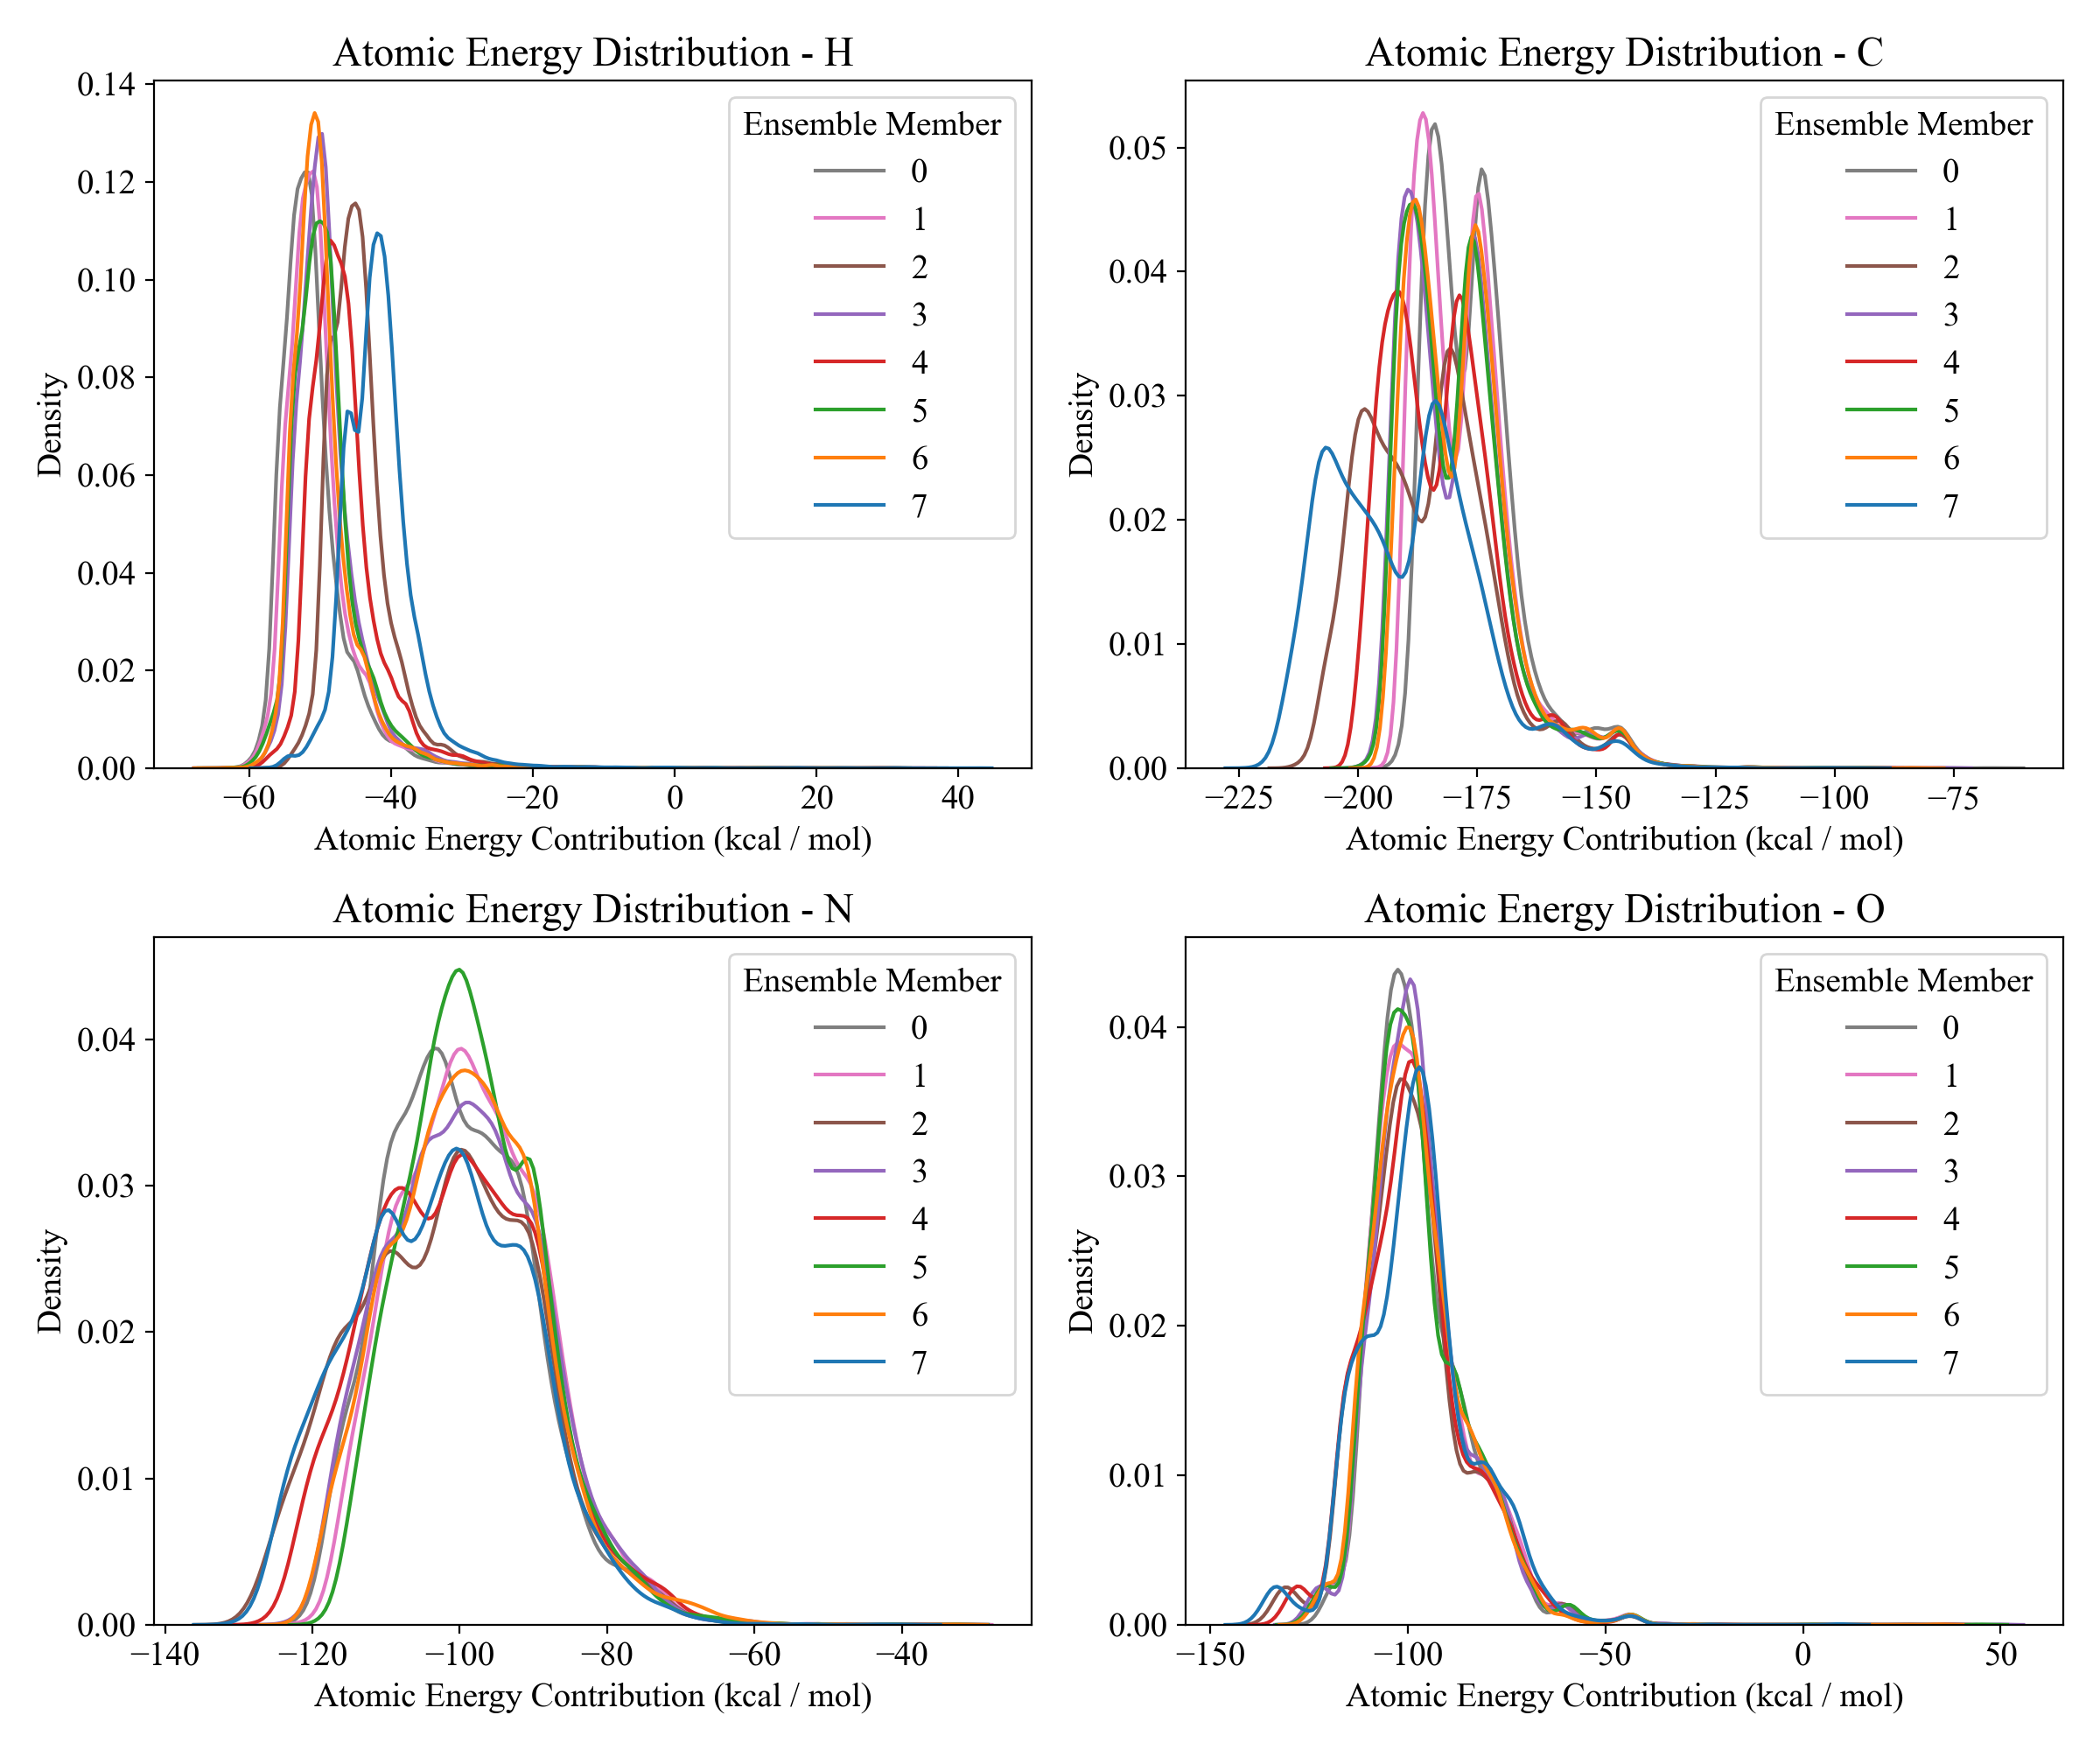
\includegraphics[width=1\linewidth]{Images/2xr_outputs/2xr_1x-first_ae-per-model.png}
    \caption[Atomic energies predicted by ANI-2xr]{Distribution of atomic energy contributions by atom type for the ANI-2xr potential. Values shown in kcal/mol for CHNO atom types on the 1x-first subset.}
    \label{fig:2xr_ae_per_model}
\end{figure}

The difference in the shapes of these distributions is an important aspect of analyzing the predictive uncertainty of ANI neural network potentials.
Due to the differences in hyperparameters used in training, such as the removal of biases, the use of the GELU activation function \cite{gelu} continuous second derivatives improving the smoothness of predicted potential energy surfaces, and the addition of ground state atomic energies and a repulsive term, ANI-2xr will be used to explore trends in uncertainty in predictions by ANI neural networks. 

\subsection{Uncertainty in ANI Neural Network Potentials}
\label{subsec:ANI_uncertainty}

ANI potential models use an ensemble of eight independently models, allowing for the estimation of predictive uncertainty.
This uncertainty metric is frequently used in active learning strategies to guide data selection for model improvement.
Predictive uncertainty has been measured in published models using $\hat{\rho}$; the value 0.23 kcal/mol was empirically chosen for sampling structures with high-error energy predictions via query by committee (QBC) in the active learning process \cite{ani-1x}.
The QBC value, given in Eqn. \ref{eq:energy_qbc}, can be thought of as a binary classifier: molecules with QBC values above 0.23 kcal/mol are highly-uncertain predictions and shouldn't be trusted, while values below 0.23 kcal/mol are trustworthy, agreed upon values by the ensemble.

\begin{equation}
\rho = \frac{\sigma_{E_{\text{Total}}}}{\sqrt{N_{\text{atoms}}}}
\label{eq:energy_qbc}
\end{equation}

This normalization accounts for the size of the molecule, ensuring that uncertainty values remain comparable across different molecular systems. 
In the development of ANI-1x, a threshold value of 0.23 kcal/mol was empirically chosen as the criterion for selecting molecules with high-energy uncertainty for further active learning \cite{ani-1x}.
However, while QBC serves as a useful uncertainty metric for guiding active learning, it introduces a size-dependent limitation. Because $\sqrt{N_\text{atoms}}$ appears in the denominator, molecules with a large number of atoms can exhibit low uncertainty values, even if individual atomic energy predictions are highly uncertain. 
This means that large structures may be misclassified as “low-error” molecules despite containing regions of high uncertainty in their atomic energy contributions. 
Consequently, high-error structures may slip through the active learning process, leading to gaps in the training data for larger molecules.

To explore this issue further, atomic energy predictions can be examined on a per-atom-type basis. 
Figure \ref{fig:2xr_comp6v1_mean-ae-per-atomtype} presents the distribution of mean atomic energy predictions using the ANI-2xr model on the COMP6v1 benchmark set. 
This per-atom decomposition allows for a finer-grained analysis of uncertainty, revealing how specific atomic environments contribute to total energy predictions and where potential weaknesses in the model may arise.

\begin{figure}[H]
    \centering
    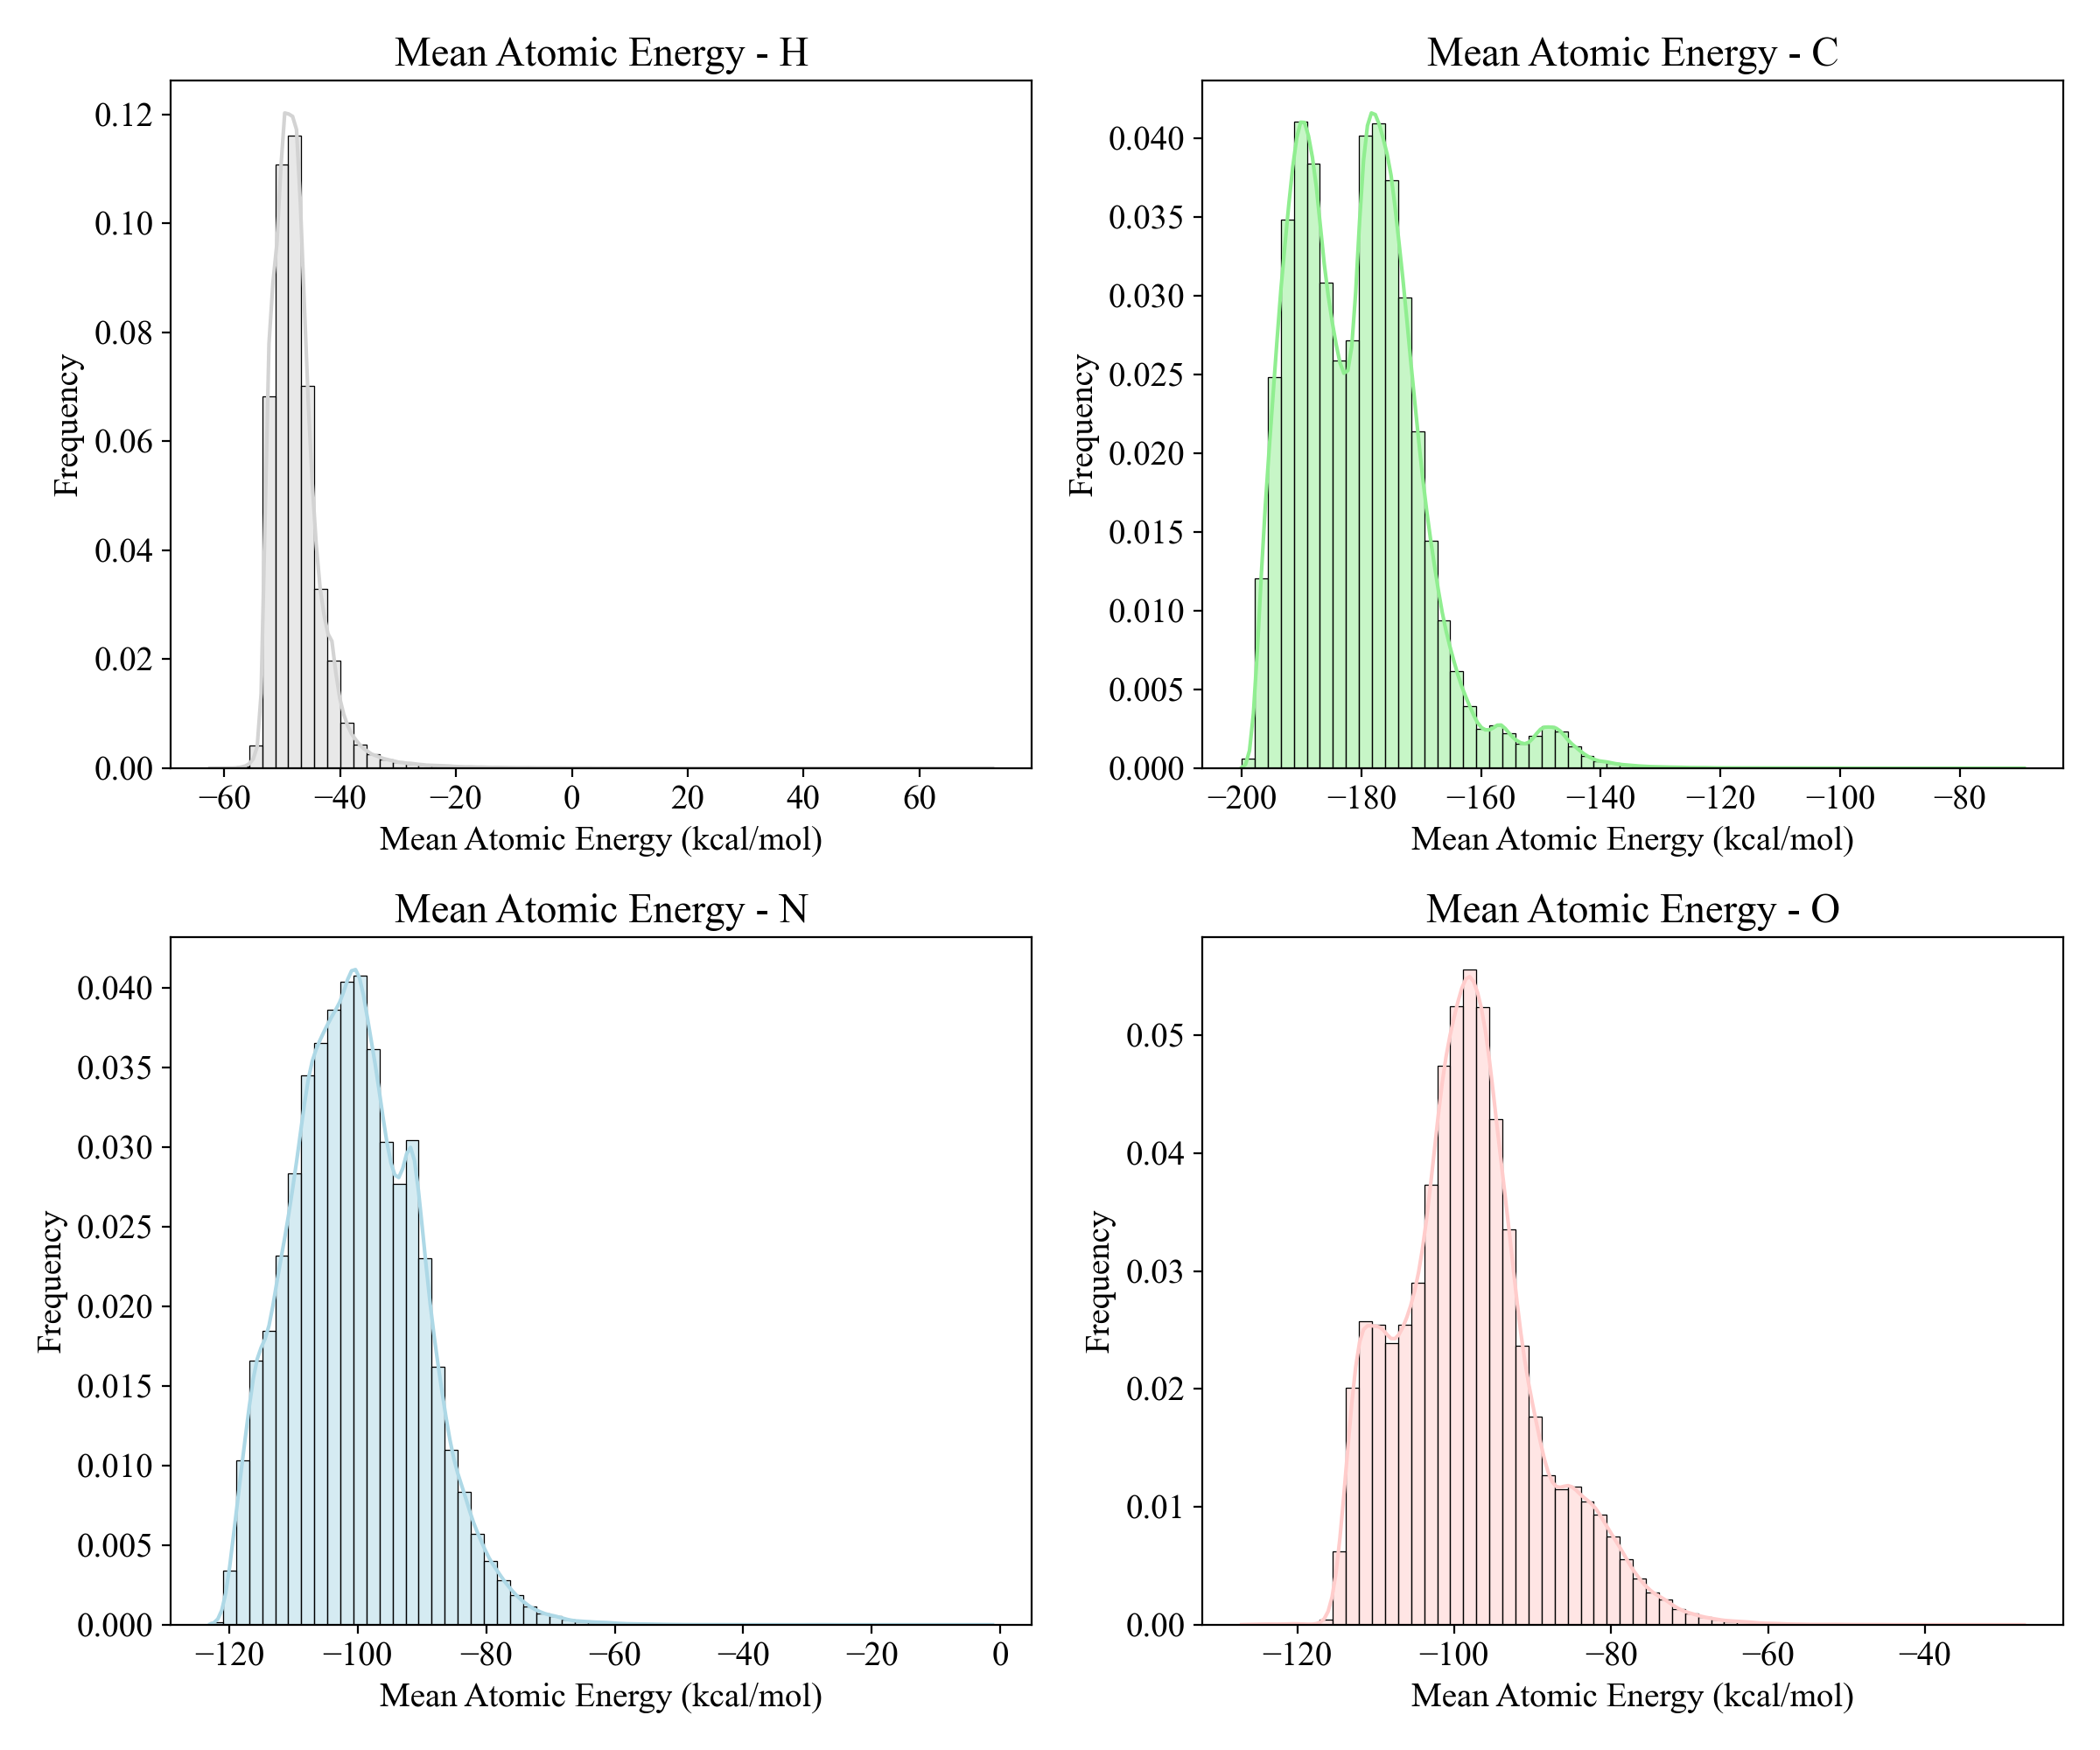
\includegraphics[width=1\linewidth]{Images/2xr_outputs/2xr_comp6v1_mean-ae-per-atomtype.png}
    \caption[Mean atomic energy prediction per-atom with ANI-2xr]{Distribution of predicted mean atomic energies using the ANI-2xr model on the COMP6v1 benchmark set.}
    \label{fig:2xr_comp6v1_mean-ae-per-atomtype}
\end{figure}

By analyzing per-atom energy contributions, it becomes possible to refine uncertainty quantification methods beyond QBC, addressing the size-dependent bias and improving the selection of high-error molecules for retraining in future ANI models.

\subsection{Exploration of the Flaws in Measuring Uncertainty via Predicted Total Energy}
\label{subsec:flaws_in_qbc}

A clear example of size dependence in ANI uncertainty estimation can be illustrated by considering a small molecule with a high query-by-committee (QBC) value. Suppose we start with a simple molecule, such as propane (C\textsubscript{3}H\textsubscript{8}), where a particular atomic region exhibits a relatively high uncertainty in its predicted atomic energies. Because QBC normalizes by the square root of the number of atoms $\left(\sqrt{N_\text{atoms}} \right)$, the uncertainty estimate is influenced heavily by molecular size.

Now, consider a structurally similar but larger molecule, \authorRemark{REWRITE THIS TO THE m-epoxide EXAMPLE ... } such as undecane (C\textsubscript{11}H\textsubscript{24}), which is derived from propane by extending one of its methyl functional groups into a 10-carbon chain. Despite this significant increase in molecular size, the region of high atomic uncertainty in the original molecule still exists—for example, in the same local chemical environment near the initial site of uncertainty. However, because $\left(\sqrt{N_\text{atoms}} \right)$ is much larger, the total molecular uncertainty value ($\rho$) is now lower, even though the model's uncertainty in that specific region has not improved.

This example demonstrates how large molecules can exhibit deceptively low QBC values, making it more difficult to identify high-error structures in active learning. As a result, potentially problematic regions of uncertainty can be overlooked in training set refinement, leading to overconfidence in predictions for large systems. Such effects highlight the need for alternative uncertainty quantification methods that account for localized atomic errors rather than relying solely on global molecular uncertainty metrics.

As the energy of molecules is predicted as a sum of atomic contributions---and therefore, one could say, the networks are actually predicting atomic energies---the first exploration into an atomistic uncertainty method was into the atomic energy contribution predicted for each atom.

\section{Uncertainty of Atomic Energy Predictions}
\label{sec:uncertainty_atomic_energies}

Predictive uncertainty in ANI neural network potentials extends beyond total molecular energy predictions, affecting atomic energy contributions on a per-atom basis. The standard deviation in atomic energy predictions across an ensemble of ANI models provides insight into how confidently the model assigns energetic contributions to individual atoms. Figure \ref{fig:2xr_comp6v1_stdev-ae-per-atomtype} illustrates the distribution of atomic energy standard deviations for different atom types (H, C, N, O) using the ANI-2x model on the COMP6v1 benchmark set. Higher uncertainty in atomic energy predictions often correlates with underrepresented chemical environments in the training data, where the model struggles to generalize beyond learned patterns. Additionally, atoms in highly strained or reactive regions tend to exhibit greater variance, reflecting the challenge of accurately capturing energy contributions in chemically complex systems.

\begin{figure}[H]
    \centering
    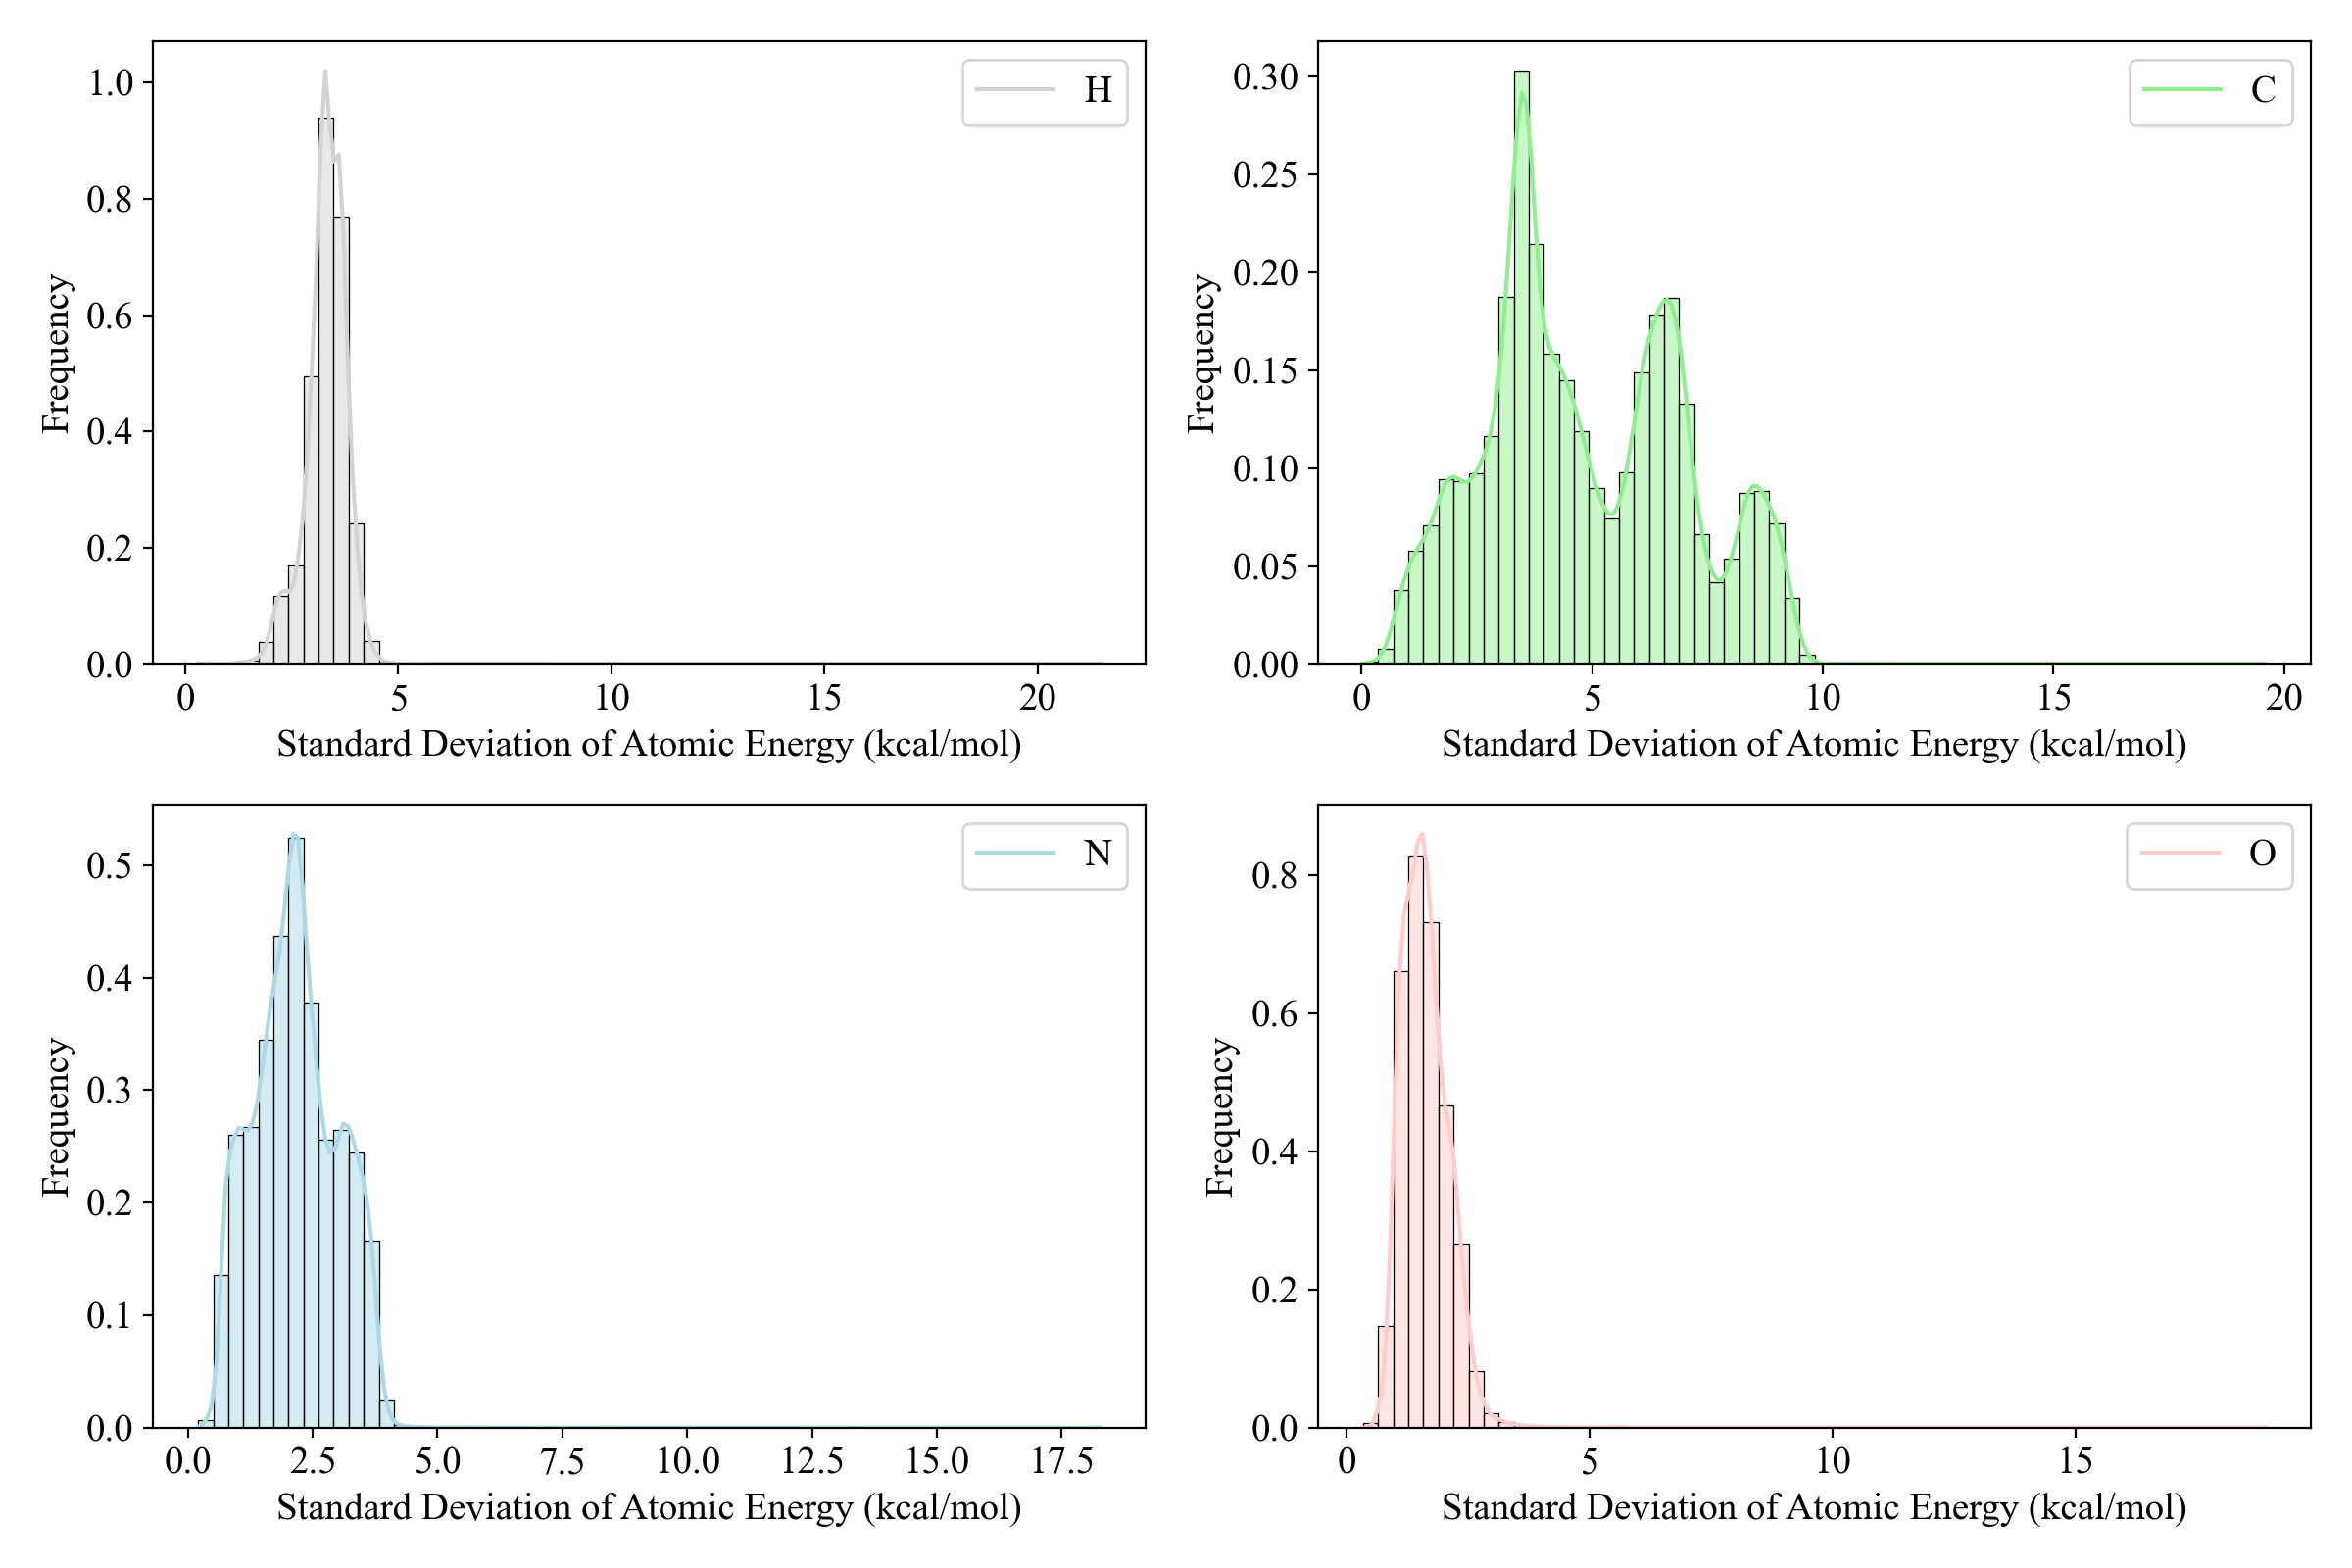
\includegraphics[width=1\linewidth]{Images/2xr_outputs/2xr_comp6v1_stdev-ae-per-atomtype.png}
    \caption[Standard deviation in predicted atomic energy contribution for H, C, N, O atom types]{Distribution of standard deviation in predicted atomic energies using the ANI-2x model on the COMP6v1 benchmark set.}
    \label{fig:2xr_comp6v1_stdev-ae-per-atomtype}
\end{figure}

Higher uncertainty in atomic energy contributions often arises in chemically complex or underrepresented environments in the training data. While carbon and oxygen atoms typically exhibit lower variance due to their frequent occurrence in organic molecules, hydrogen atoms display a broader spread, reflecting their dependence on local bonding environments. This is particularly relevant in systems where heteroatoms or extended conjugation patterns influence local electronic structure, leading to higher variability in atomic energy assignments.
An illustrative example of this phenomenon can be seen in methane (CH\textsubscript{4}), which is a highly symmetric molecule with four chemically equivalent hydrogen atoms and a single carbon center. Figure \ref{fig:ch4_stdev_ae} presents the standard deviation in atomic energy contributions for CH\textsubscript{4} across the ANI-2xr model ensemble, compared to the total energy uncertainty distribution in the 1x-first test set.

\begin{flushleft}
\begin{multiFigure}
    \addFigure{0.31}{Images/ch4.png}
    \addFigure{0.68}{Images/ch4_example/ch4_2xr_total-e-qbc.png} \\
    \addFigure{1}{Images/ch4_example/ch4_2xr_stdev-ae.png}
\captionof{figure}[CH\textsubscript{4} atomic energy distribution vs 1x-first]{
(A) Structure of geometry-optimized CH\textsubscript{4}; 
(B) Plot of the distribution of total energy QBC across the 1x-first test set, 
(C) standard deviation in predicted atomic energy for hydrogen (left) and carbon (right); 
the red lines show the standard deviation in CH\textsubscript{4} total energy (B) and atomic energy contributions (C).
}
\label{fig:ch4_stdev_ae}
\end{multiFigure}
\end{flushleft}

While total molecular energy predictions for CH\textsubscript{4} remain relatively low in uncertainty, the per-atom standard deviations reveal higher variability in atomic energy contributions, particularly in hydrogen. This suggests that even in highly symmetric molecules, ANI's per-atom energy assignments may be non-trivial, introducing potential sources of error in energy decomposition analyses.

The per-atom uncertainty in ANI models is not only influenced by the training data but also by learned covariances across network predictions. The atomic energy contributions predicted by different models within the ANI ensemble exhibit correlated variations, where changes in one atomic energy may be systematically offset by adjustments in another.
For example, Table \ref{tbl:ch4_AEs} reports the atomic energy contributions predicted by each model in the ANI-2xr ensemble for CH\textsubscript{4}. While the individual atomic energies fluctuate across models, the sum of atomic energies remains tightly constrained, with a standard deviation an order of magnitude lower than that of the individual atomic contributions.

% Tables suck, but this helped me align columns and headers separately:
\begin{table}[hbt]
\centering
\caption[CH\textsubscript{4} atomic energy contributions per-model]{
Atomic energy contributions by atom type in a geometry-optimized molecule of CH\textsubscript{4}, with four equivalent hydrogen atoms. 
Additionally, the sum over all atoms, and that sum after passing through the TorchANI EnergyShifter. 
Values obtained from an ensemble of ANI models (ANI2xr); the last column shows the standard deviation of predictions across the ensemble. 
All values are in kcal/mol.
}\label{tbl:ch4_AEs}
    \begin{tabularx}{\textwidth}{%
    >{\raggedleft\arraybackslash}r  % Numeric
    >{\raggedleft\arraybackslash}r  % Numeric
    >{\raggedleft\arraybackslash}r  % Numeric
    >{\raggedleft\arraybackslash}r  % Numeric
    >{\raggedleft\arraybackslash}r  % Numeric
    }  
\hline
Model & Carbon & Hydrogen  & Sum of atomic energies & Molecular energy \\
\hline
Mean prediction & -199.0069 & -55.1013 & -419.4123 & -25413.8125 \\
1 & -219.4329 &  -50.0170 &  -419.5012 &  -25413.9043 \\
2 & -194.7117 &  -56.1991 &  -419.5081 &  -25413.9102 \\
3 & -192.8823 &  -56.6466 &  -419.4689 &  -25413.8691 \\
4 & -201.5683 &  -54.4451 &  -419.3490 &  -25413.7500 \\
5 & -196.5227 &  -55.7060 &  -419.3471 &  -25413.7500 \\
6 & -212.9323 &  -51.5945 &  -419.3103 &  -25413.7109 \\
7 & -186.5623 &  -58.2018 &  -419.3694 &  -25413.7715 \\
8 & -187.4427 &  -58.0003 &  -419.4441 &  -25413.8457 \\
Standard deviation &  11.7621 &  2.9412 &  0.0775 &  0.0775 \\
\hline
\end{tabularx}
\end{table}

This covariance, defined in Eqn. \ref{eq:covariance}, reflects a learned compensation mechanism where certain atomic energy predictions systematically adjust in response to others.

\begin{equation}
    \label{eq:covariance}
    \text{cov}(x, y) = \mathbb{E}[(x - \mathbb{E}[x])(y - \mathbb{E}[y])]
\end{equation}

This suggests that ANI models learn relative atomic energy distributions, where variations in one atom's contribution are counterbalanced by adjustments in others to maintain a stable total molecular energy. To better understand this effect, Figure \ref{fig:ch4_covariance} presents covariance matrices of atomic energy contributions for CH\textsubscript{4} and pentane (C\textsubscript{5}H\textsubscript{12}), highlighting correlation patterns between atomic contributions in molecules of different sizes.

\begin{flushleft}
\begin{multiFigure}
    \addFigure{0.2}{Images/covariance/ch4_labeled.png}
    \addFigure{0.65}{Images/covariance/ch4_covariance.png}
    \addFigure{0.28}{Images/covariance/c5h12_labeled}
    \addFigure{0.65}{Images/covariance/c5h12_covariance.png} \\
\captionof{figure}[Atomic energy covariance matrices]{
(A) Geometry-optimized structure of CH\textsubscript{4}; 
(B) Matrix visualizing the covariance of atomic energies predicted by ANI-2xr for this structure of CH\textsubscript{4}; 
(C) Structure of geometry-optimized C\textsubscript{5}H\textsubscript{12}; 
(D) Covariance matrix for predicted atomic energies of C\textsubscript{5}H\textsubscript{12}.}
\label{fig:ch4_covariance}
\end{multiFigure}
\end{flushleft}

This compensatory behavior suggests that ANI models do not learn absolute atomic energies in isolation, but rather relative energy distributions that maintain a consistent total molecular energy. As a result, variations in one atomic contribution are often counterbalanced by adjustments in neighboring atoms, preserving overall energetic stability while allowing individual atomic predictions to fluctuate.
These covariance effects contribute to the observed size dependence in ANI model uncertainty, where molecular energy predictions remain stable while per-atom uncertainties fluctuate.
This behavior is due to learned covariances across networks, where, for example, carbon atomic energies learn to offset hydrogen energy contributions in the training process. This relationship is defined in Eqn. \ref{eq:total_e_covariance}.

\begin{equation}
    \sigma_{E_{\text{total}}}^2 = \sum_i^{N \text{ (atoms)}} \sigma_{E_{\text{atomic}}}^2 + 2 \sum_i^N \sum_{j \neq i}^N \text{cov}(x_i, y_j) = \sum_{i,j}^N \text{cov}(x_i, x_j)
    \label{eq:total_e_covariance}
\end{equation}

This covariance-driven redistribution of uncertainty is a key challenge in using ANI for uncertainty-aware simulations, as it impacts force predictions, molecular dynamics stability, and error estimation in out-of-sample predictions.

\section{Need for a Practical, Physical Quantity to Estimate Uncertainty}
\label{sec:practical_physical_quantity_for_uncertainty}

The predictive uncertainty in ANI models has primarily been examined through atomic energy distributions, but these values lack intrinsic physical meaning beyond their role in reproducing the total molecular energy. A fundamental limitation of atomic energy assignments is their model dependence—each of the eight neural networks in the ensemble learns a slightly different decomposition of molecular energy, leading to inconsistencies in per-atom contributions. This variability makes atomic energies ill-suited as a reliable uncertainty measure, as they do not correspond to an independently verifiable physical property.

A more robust alternative lies in atomic forces, which ANI models also predict as derivatives of the potential energy surface, shown in Equation \ref{eq:force_dE}. 
\begin{equation}
    \vec{F} = -\nabla E
    \label{eq:force_dE}
\end{equation}

Unlike atomic energies, forces directly correspond to the physical structure and motion of molecules, as they describe how atoms interact under the influence of a potential. Forces dictate molecular geometry, vibrational frequencies, reaction pathways, and dynamics, making them a natural choice for evaluating model reliability. Since ANI is trained to approximate the true quantum mechanical PES, its force predictions serve as an indirect measure of how well the model captures the curvature of the PES, providing insight into both local stability and model confidence.

The combined energy and force loss function used in ANI training, given in Eqn. \ref{eq:force_loss}, minimizes the molecular energy error while also penalizing discrepancies in predicted atomic forces. This introduces an additional constraint that enhances the physical reliability of the learned potential energy surface:

\begin{equation}
\mathcal{L}_{\text{E \& }\vec{\text{F}}} = 
\frac{1}{N_{\text{M}}} 
\sum_{i=1}^{N_\text{M}} 
\left[ \left( \frac{
\left( E_{\text{ANI}}^{\text{o},i} - E_{\text{QM}}^{\text{o},i} \right)^2}
{\sqrt{N_{\text{atoms}}}} \right)
+ 0.1 \ast \left( 
\frac{\sum_{j=1}^{N_{\text{atoms}}} 
\left( \vec{f}_{\text{ANI}}^{j} - \vec{f}_{\text{QM}}^{j}\right)^2}{N_{\text{atoms}}} 
\right) \right]
\label{eq:force_loss}
\end{equation}

This loss function consists of two key components that work together to optimize both molecular energy and atomic force predictions. The first component addresses energy loss by computing the mean squared error (MSE) between the predicted molecular energy and the reference quantum mechanical energy. To ensure that large molecules do not disproportionately influence the optimization process, the loss is normalized by the square root of the number of atoms in the system. This normalization maintains consistency in model performance across different molecular sizes. The second component focuses on force loss, which is calculated as the difference between the predicted atomic forces and the quantum mechanical reference forces. Since each atom experiences forces that determine molecular motion and stability, the force loss is averaged over all atoms in the molecule, treating each force vector as an independent target for training. To balance the contributions of energy and force errors, a scaling factor of 0.1 is introduced, preventing one component from dominating the learning process. This ensures that the model refines both energy and force predictions simultaneously, leading to a more physically meaningful representation of molecular interactions.

By training ANI to predict forces along with energies, we gain access to a physically meaningful metric for uncertainty estimation. Since forces describe how gradients of the potential energy surface vary across atomic positions, their accuracy directly reflects the model's ability to approximate quantum mechanical interactions.
When an ANI model encounters a molecule outside of its training distribution, its force predictions may become erratic or inconsistent across the ensemble, reflecting the model’s lack of confidence in extrapolating beyond familiar chemical environments. By analyzing the standard deviation in force predictions across the ANI ensemble, we can construct a size-independent measure of uncertainty that is directly tied to physical observables rather than arbitrary atomic energy assignments.
This insight forms the foundation for the next chapter, where we explore how force-based uncertainty metrics can be used to assess ANI model reliability in molecular simulations, and how these methods compare to traditional QBC-based energy uncertainty approaches.